\documentclass[11pt,class=report,crop=false]{standalone}
\usepackage{exo7hilisit}

\begin{document}


\entete{Hilisit}{Capacité mathématiques}

\titre{\'Equations différentielles -- Partie 4 : $\boldsymbol{y'=ay+b}$ et $\boldsymbol{y'=ay+f}$} 

\bigskip
\bigskip


%%%%%%%%%%%%%%%%%%%%%%%%%%%%%%%%%%%%%%%%%%%%%%%%%%%%%%%%%%%%
%\section{$y'=ay+b$ et $y'=ay+f$}

\exercice{}
\enonce
Pour chacune des équations différentielles $(E)$ suivantes, 
 \begin{itemize}
  \item déterminer l'équation homogène associée,
  \item trouver les solutions $y_h(x)$ de cette équation homogène,
  \item vérifier que la fonction $y_p(x)$ est bien solution de l'équation différentielle $(E)$,
  \item en déduire toutes les solutions de $(E)$.
\end{itemize} 
 
 \begin{enumerate}
  \item $y'=-y+x^2+1$, $y_p(x)=x^2-2x+3$
  \item $y'=y+2\cos(x)$, $y_p(x)=\sin(x)-\cos(x)$ 
  \item $y'=3y+xe^{2x}$, $y_p(x)=-(x+1)e^{2x}$
\end{enumerate} 
\finenonce

\indication
Pour une équation différentielle $(E)$ : $y' = ay + f$, l'équation homogène est $y'=ay$. Si l'on note les solutions de l'équation homogène $y_h$, et une solution particulière de $(E)$ $y_p$, alors toutes les solutions de $(E)$ sont les fonctions $y_h + y_p$.
\finindication


\correction
\sauteligne
 \begin{enumerate}
  \item 
  $(E_h) : y'=-y$, $y_h(x) = Ce^{-x}$,
  $(E) : y'=-y+x^2+1$, dont $y_p(x)=x^2-2x+3$ est une solution particulière puisque $y_p'(x) = 2x-2 = -(x^2-2x+3) + x^2 + 1 = -y_p(x) + x^2 + 1$. Les solutions générales de $(E)$ sont les $y(x) = y_h(x)+y_p(x)=Ce^{-x}+x^2-2x+3$ où $C$ est une constante réelle.

  \item 
  $(E_h) : y'=y$, $y_h(x) = Ce^{x}$,
  $(E) : y'=y+2\cos(x)$, dont $y_p(x)=\sin(x)-\cos(x)$ est une solution particulière. Les solutions générales de $(E)$ sont les $y(x) = y_h(x)+y_p(x)=Ce^{x}+\sin(x)-\cos(x)$ où $C$ est une constante réelle.

  \item 
  $(E_h) : y'=3y$, $y_h(x) = Ce^{3x}$,
  $(E) : y'= 3y + x e^{2x} $, dont $y_p(x)= -(x+1)e^{2x}$ est une solution particulière. Les solutions générales de $(E)$ sont les $y(x) = y_h(x)+y_p(x)=Ce^{3x}-(x+1)e^{2x}$ où $C$ est une constante réelle.

\end{enumerate} 
\fincorrection
\finexercice

\exercice{}
\enonce
Pour chacune des équations différentielles $(E)$ suivantes, 
 \begin{itemize}
  \item déterminer l'équation homogène associée,
  \item trouver les solutions $y_h(x)$ de cette équation homogène,
  \item trouver une solution particulière $y_p(x)$ en vous aidant des indications,
  \item en déduire toutes les solutions de $(E)$.
\end{itemize} 
 
 \begin{enumerate}
  \item $y'+2y=5$, chercher une solution particulière sous la forme d'une fonction constante.  % 5
  \item $2y'-3y=e^{-x}$, chercher une solution particulière sous la forme $ke^{-x}$ où $k$ est une constante à déterminer. % -1/5e^{-x}$
  \item $y'=y + x^2$, chercher une solution particulière sous la forme $ax^2+bx+c$.    % - x^2 - 2 x - 2
\end{enumerate} 
\finenonce

\indication
Pour une équation différentielle $(E)$ : $y' = ay + f$, l'équation homogène est $y'=ay$. Si l'on note les solutions de l'équation homogène $y_h$, et une solution particulière de $(E)$ $y_p$, alors toutes les solutions de $(E)$ sont les fonctions $y_h + y_p$.
\finindication

\correction
\sauteligne
 \begin{enumerate}
  \item 
  Équation homogène : $y' + 2y = 0$ soit $y' = -2y$.\\
  Solutions de l'équation homogène : $y_h(x) = Ce^{-2x}$.\\
  Solution particulière constante : $y_p(x)= \frac 5 2$.\\ 
  Solutions générales : $y(x) = y_h(x) + y_p(x) = Ce^{-2x} + \frac 5 2$ où $C$ est une constante réelle.

  \item 
  Équation homogène : $2y'-3y = 0$ soit $y' = \frac 32 y$.\\
  Solutions de l'équation homogène : $y_h(x) = Ce^{\frac32x}$.\\
  Solution particulière : $y_p(x) = -\frac15 e^{-x}$.\\ 
  Solutions générales : $y(x) = y_h(x) + y_p(x) = Ce^{\frac32x}-\frac15 e^{-x}$ où $C$ est une constante réelle.

  \item 
  Équation homogène : $y' = y$.\\
  Solutions de l'équation homogène ; $y_h(x) = Ce^{x}$.\\
  Solution particulière : $y_p(x) = - x^2 - 2 x - 2$.\\ 
  Solutions générales : $y(x) = y_h(x) + y_p(x) = Ce^{x} - x^2 - 2 x - 2$ où $C$ est une constante réelle.
\end{enumerate} 
\fincorrection
\finexercice




\exercice{}
\enonce

Le dessin représente quelques solutions de l'équation différentielle $(E) : y'=2y+x^2e^x$.

\begin{center}
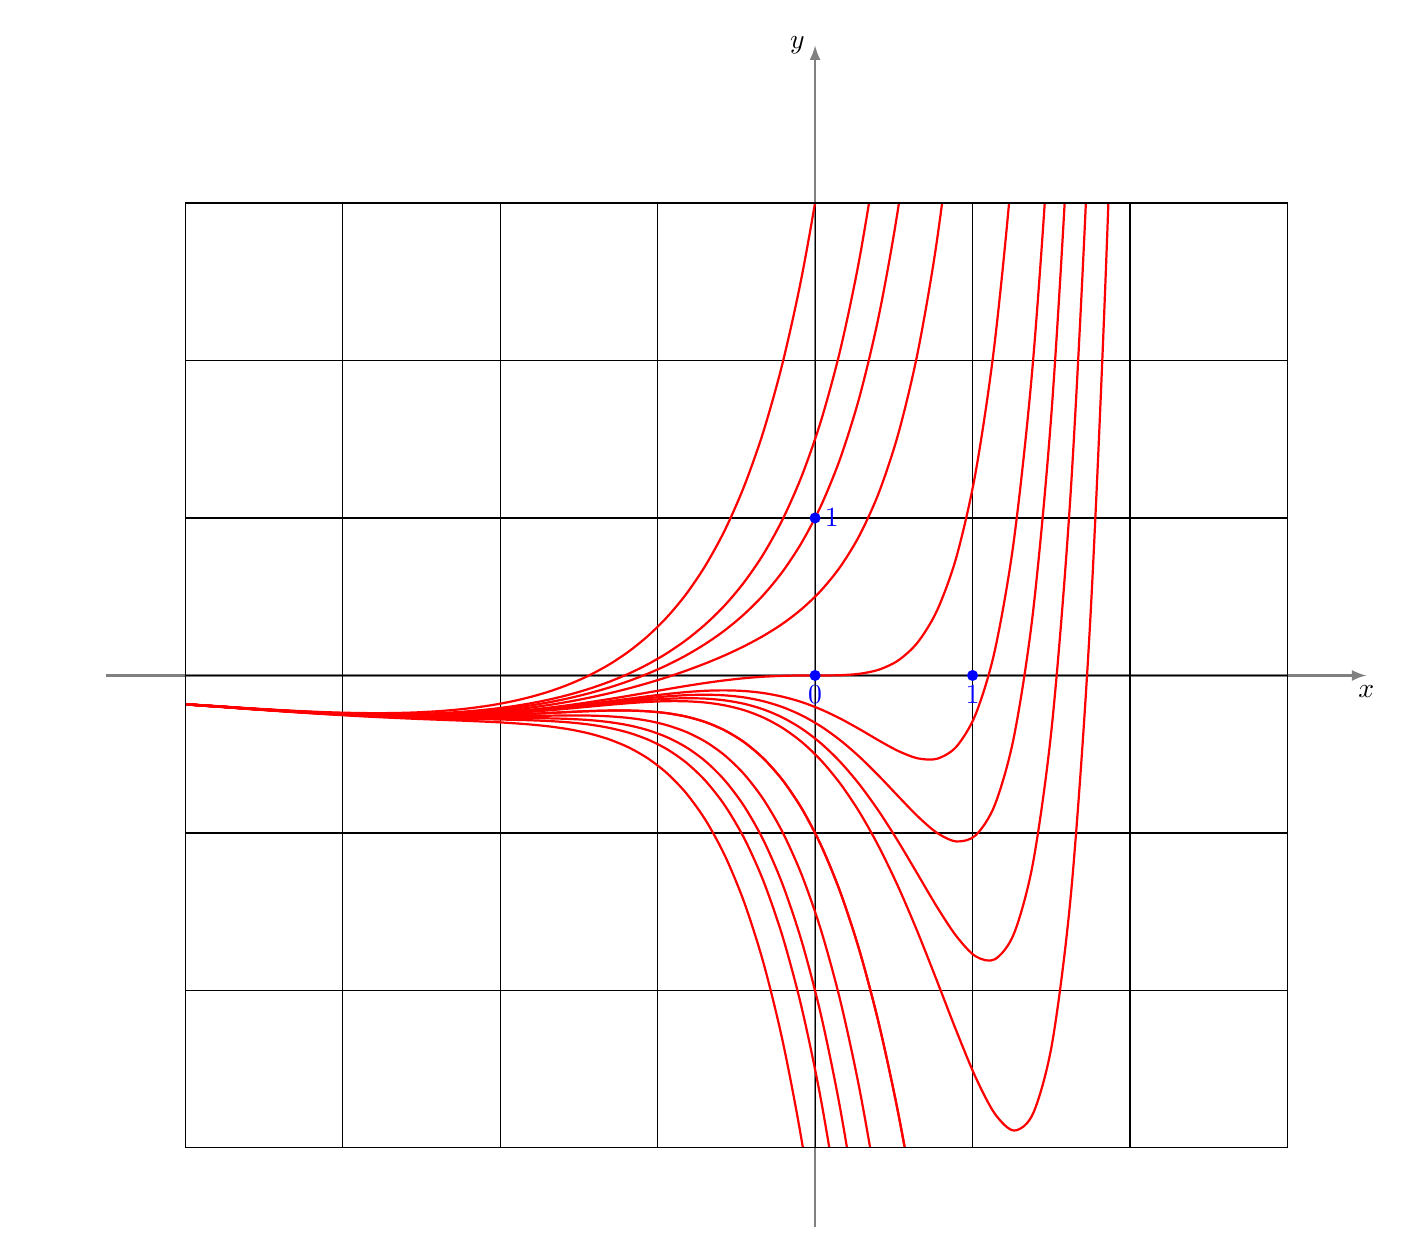
\begin{tikzpicture}[scale=2]

  \draw[->,>=latex,thick,gray] (-4.5,0) -- (3.5,0) node[below,black] {$x$};
  \draw[->,>=latex,thick,gray] (0,-3.5) -- (0,4) node[left,black] {$y$};
  \draw (-4,-3) grid (3,3);
\begin{scope}
    \clip (-5,-3) rectangle (3,3);


\foreach \k in {-1.5,-0.5,0,1,0.5,1,1.5,1.6,1.7,1.8,2,2.5,3,3.5,5} {
  \draw[thick, color=red,domain=-4:2, smooth, samples=50] plot (\x,{\k*exp(2*\x)-((\x)^2+2*\x+2)*exp(\x)}); 
}

\end{scope}

\fill[blue] (0,0)  circle (1pt) node [below] {$0$}; 
\fill[blue] (1,0)  circle (1pt) node [below] {$1$}; 
\fill[blue] (0,1)  circle (1pt) node [right] {$1$};

\draw (-4,-3) rectangle (3,3);

\end{tikzpicture}
\end{center}


\begin{enumerate}
  \item Tracer la tangente à la courbe solution qui passe par le point $(0,0)$. Retrouver son équation par le calcul  grâce à l'équation différentielle.

  \item Tracer la tangente à la courbe solution qui passe par le point $(0,1)$. Retrouver son équation par le calcul grâce à l'équation différentielle.

  \item Tracer la tangente à la courbe solution qui passe par le point $(1,-1)$. Retrouver son équation par le calcul grâce à l'équation différentielle.

  \item Déterminer les solutions $y_h(x)$ de l'équation homogène.

  \item Déterminer une solution particulière $y_p(x)$ sous la forme $(ax^2+bx+c)e^x$.

  \item En déduire toutes les solutions de $(E)$.

\end{enumerate} 
\finenonce

\noindication

\correction
\sauteligne
\begin{enumerate}
  \item Par lecture graphique il semble que la tangente en $(0,0)$ soit horizontale. Vérifions-le par le calcul. La solution $f$ dont le graphe passe par $(0,0)$ vérifie $f(0)=0$. Comme $f$ vérifie l'équation différentielle $y'=2y+x^2e^x$, alors $f'(0)=2f(0)+0^2\cdot e^0=0$, donc la tangente est bien horizontale. Son équation est $y=0$.

  \item La solution $g$ dont le graphe passe par $(0,1)$ vérifie $g(0)=1$. Comme $g$ vérifie l'équation différentielle alors $g'(0)=2g(0)+0^2\cdot e^0=2$, donc la pente de la tangente est $2$ et son équation est $y=2x+1$.

  \item La solution $h$ dont le graphe passe par $(1,-1)$ vérifie $h(1)=-1$. Comme $h$ vérifie l'équation différentielle alors $h'(1)=2h(1)+1^2\cdot e^1=e-2$, donc la pente de la tangente est $e-2$ et comme cette droite passe par $(1,-1)$ son équation est $y=(e-2)(x-1)-1$, c'est-à-dire $y=(e-2)x+1-e$.

  \item L'équation homogène est $(E_h) : y'=2y$, dont les solutions sont $y_h(x) = Ce^{2x}$, pour toute constante réelle $C$.

  \item Cherchons une solution particulière sous la forme $y_p(x) = (ax^2+bx+c)e^x$. Alors $y'_p(x) = (ax^2+(2a+b)x+b+c)e^x$.
  \begin{align*}
        & y_p(x) \text{ solution de } (E) \\
   \iff & y_p'(x) =2y_p(x) +x^2e^x  \text{ pour tout } x \in \Rr \\
   \iff & (ax^2+(2a+b)x+b+c)e^x =2(ax^2+bx+c)e^x +x^2e^x \\
   \iff & e^x\big((a+1)x^2 + (b-2a)x + (c-b) \big)  = 0 \\
   \iff & (a+1)x^2 + (b-2a)x + (c-b)  = 0 \qquad \text{car } e^x \neq 0 \\
   \iff & a+1 = 0 \quad \text{ et } \quad b-2a = 0 \quad \text{ et } \quad c-b = 0 \\
   \iff & a=-1, b=-2, c=-2 \\
  \end{align*}
   Ainsi $y_p(x) =  (-x^2 - 2x - 2)e^x = -(x^2+2x+2)e^x$ est une solution particulière.

  \item Les solutions générales de $(E)$ sont $y(x) = y_h(x) + y_p(x) = Ce^{2x} - (x^2 + 2 x + 2)e^x$ où $C$ est une constante réelle.
\end{enumerate} 
\fincorrection
\finexercice


\end{document}
